% Main entry for OS project documentation (ctex + custom style)
\documentclass[12pt,oneside]{ctexbook}

% Project custom style
\usepackage{style/custom}

% Metadata
\newcommand{\ProjectName}{Your OS}
\newcommand{\DocVersion}{v0.1}

\title{操作系统项目工程文档\\\large 基于自制内核}
\author{Your Name}
\date{\today}

\begin{document}
\maketitle
\tableofcontents

% -------------------- Preface --------------------
\frontmatter
\chapter*{前言}
\addcontentsline{toc}{chapter}{前言}

这是一套基于 \textbf{ctexbook} 与自定义样式的工程/教材级文档骨架,目标是:

- 美观、易读,适合“书籍式”通读;
- 代码高亮丰富(优先 \texttt{minted},可自动降级到 \texttt{listings});
- 结构清晰,便于长期维护与扩展;
- 与仓库保持紧密联系,支持直接引用源码文件。

\begin{qsbox}[title=快速开始]
在 \texttt{doc/} 目录执行:\texttt{latexmk};PDF 输出位于 \texttt{\_build/main.pdf}。若系统缺少 \texttt{minted},将自动使用 \texttt{listings}。
\end{qsbox}


% -------------------- Main matter --------------------
\mainmatter
\chapter{引导程序}

本章围绕仓库中 \mintinline{text}{boot/} 目录的实现展开,梳理从主引导记录(MBR)到 Loader 的完整流程:磁盘布局、实模式初始化、LBA 读盘、内存探测、进入保护模式以及为内核准备分页环境。重点解释高半区(0xC0000000 以上)执行所需的指令与数据布局。

\section{磁盘布局与常量约定}

引导阶段的内存与磁盘布局通过 \mintinline{text}{boot/include/boot.inc} 统一声明,涵盖 Loader 与内核的加载地址、分页用到的物理页框等常量:

\begin{table}[h]
    \centering
    \begin{tabular}{lll}
        \toprule
        标识符 & 含义 & 数值/扇区号 \\
        \midrule
        \mintinline{text}{LOADER_BASE_ADDR} & Loader 复制到内存的基址 & 0x900 (实模式可用) \\
        \mintinline{text}{LOADER_START_SECTOR} & Loader 在磁盘的起始 LBA 扇区 & 0x2 \\
        \mintinline{text}{KERNEL_BIN_BASE_ADDR} & 保护模式下临时存放 \mintinline{text}{kernel.bin} 的内存地址 & 0x70000 \\
        \mintinline{text}{KERNEL_START_SECTOR} & 内核镜像的磁盘起始扇区 & 0x9 \\
        \mintinline{text}{PAGE_DIR_TABLE_POS} & 建立分页结构使用的物理地址 & 0x0010\,0000 (1MB) \\
        \mintinline{text}{KERNEL_ENTRY_POINT} & 最终跳转到的内核虚拟地址入口 & 0xC0001500 \\
        \bottomrule
    \end{tabular}
    \caption{引导阶段关键常量,节选自 \mintinline{text}{boot/include/boot.inc}}
\end{table}

这些约定决定了后续章节中的地址推导:MBR 负责把 Loader 复制到 0x900,Loader 则在保护模式下把内核镜像搬运至 0x70000,并在分页开启后跳到 0xC0001500。



\section{复位向量与 BIOS 启动模型}

CPU 上电后从 \mintinline{text}{CS:IP=0xF000:0xFFF0}(物理地址 0xFFFF0)取指,执行 BIOS 固化代码完成 POST、自检与启动设备选择,随后把选中磁盘的 LBA0 扇区读入物理地址 0x7C00 并跳转。此时处理器处于 16 位实模式(分段寻址 \mintinline{text}{phys = 16*seg + off}),中断向量表位于 0:0。

\begin{notebox}[title=实模式小抄]
\begin{itemize}
  \item 段寄存器(CS/DS/ES/SS/FS/GS)均以 16 字节为粒度参与寻址:\mintinline{text}{phys = seg << 4 + off}。
  \item BIOS 提供常用中断:\mintinline{text}{int 0x10}(显示)、\mintinline{text}{int 0x13}(磁盘)、\mintinline{text}{int 0x15}(内存服务/E820)。
\end{itemize}
\end{notebox}

\section{MBR 布局速览}

主引导记录(MBR)占据磁盘第 0 个扇区(512B),布局如下:

\begin{longtable}{lll}
\toprule
偏移 & 大小 & 含义 \\
\midrule
0x000 & 446B & 启动代码(本项目:读取 Loader 至 0x900 并跳转) \\
0x1BE & 64B  & 分区表(4×16B,未在本项目解析) \\
0x1FE & 2B   & 启动签名 0x55AA \\
\bottomrule
\end{longtable}

本项目不依赖分区表,直接用常量 \mintinline{text}{LOADER_START_SECTOR=0x2} 指向 Loader 的起始扇区。

\section{执行流程概览}

在展开 MBR 细节之前,先给出从“上电”到“进入内核”的鸟瞰流程。仓库采用固定磁盘布局(MBR 位于 LBA0,Loader 从 LBA2 开始,内核从 LBA9 起),并在高半区(0xC0000000 以上)运行内核。

\begin{qsbox}[title=从上电到内核(Quick Overview)]
\begin{enumerate}
  \item 上电与 POST:BIOS 初始化最小硬件与中断向量表。
  \item 加载 MBR:BIOS 将 LBA0 读到 0x7C00 并跳转执行。
  \item MBR(16 位):统一段寄存器、显示启动标识,按 \mintinline{text}{LOADER_START_SECTOR}(默认 0x2)读取 Loader 至 0x900,跳转到 0x900:0x300。
  \item Loader(实模式):调用 \mintinline{text}{int 0x15}(优先 E820)探测物理内存,记录可用内存范围。
  \item 切换到保护模式:开启 A20,装载 GDT,设置 \mintinline{text}{CR0.PE=1},通过远跳转进入 32 位环境。
  \item 读取内核镜像:将 \mintinline{text}{kernel.bin} 自 \mintinline{text}{KERNEL_START_SECTOR}(默认 0x9)读入 0x70000 临时缓冲区。
  \item 解析并搬运:遍历 ELF Program Header,将各段复制到目标物理地址,为高半区执行做准备。
  \item 建立分页:在 1MB 处创建页目录与页表,使 PDE[0] 与 PDE[768] 指向同一张页表(低端同址映射 + 高半区镜像),最后一项指向自身以便递归映射。
  \item 开启分页与栈调整:写 \mintinline{text}{CR3},置位 \mintinline{text}{CR0.PG},把栈与数据段切换到高半区。
  \item 跳入内核:跳转到 \mintinline{text}{KERNEL_ENTRY_POINT}(0xC0001500),进入 C/C++ 内核初始化流程。
\end{enumerate}
\end{qsbox}

为便于查阅,表 \ref{tab:boot-stages} 汇总了各阶段的执行模式、入口与核心职责。

\begin{table}[h]
  \centering
  \caption{引导阶段总览}
  \label{tab:boot-stages}
  {\small
  \setlength{\tabcolsep}{6pt}
  \begin{tabularx}{\linewidth}{lll>{\raggedright\arraybackslash}X}
    \toprule
    阶段 & 模式 & 入口/地址 & 核心职责 \\
    \midrule
    BIOS & 实模式 & 加载到 0x7C00 & 读 LBA0 至 0x7C00,跳转 \\
    MBR  & 实模式 & 0x7C00 & 读 Loader 至 0x900,跳转 \\
    Loader(实→保) & 16→32 位 & 0x900:0x300→保护模式 & 内存探测、GDT、A20、读内核、建页表、开分页 \\
    Kernel & 高半区 & 0xC0001500 & 早期初始化(中断、内存管理等) \\
    \bottomrule
  \end{tabularx}}
\end{table}


\section{MBR:实模式初始化与 Loader 载入}

MBR 在 BIOS 把扇区装载到 0x7C00 后开始执行。本节将其拆分为更小的步骤逐一说明。

\subsection*{统一段寄存器与栈}
把 DS/ES/SS/FS 统一到 CS,并把栈指针设到 0x7C00,确保后续访问和调用环境稳定:

\codefilerange{nasm}{../boot/mbr.asm}{5}{12}

\subsection*{绑定 GS 指向文本显存}
将 GS 指向 0xB800 文本模式显存,便于直接写字符用于早期可视化调试:

\codefilerange{nasm}{../boot/mbr.asm}{13}{14}

\subsection*{清屏}
调用 BIOS 0x10(上卷屏幕)快速清空 25×80 文本区:

\codefilerange{nasm}{../boot/mbr.asm}{16}{22}

\subsection*{显示启动标识}
在显存首部写入“KKKZBH”,用于确认 MBR 已接管执行权:

\codefilerange{nasm}{../boot/mbr.asm}{23}{41}

\subsection*{读取 Loader 并跳转}
利用常量 \mintinline{text}{LOADER_START_SECTOR} 与 \mintinline{text}{LOADER_BASE_ADDR},读入四个扇区到 0x900,并跳到 0x900:0x300:

\codefilerange{nasm}{../boot/mbr.asm}{43}{49}

至此,控制权转交给功能更丰富的 Loader。

\section{16 位 LBA 读盘例程}

\mintinline{text}{rd_disk_m_16} 封装了 ATA 主通道的 PIO 读取流程,可分四步理解:

\subsection*{入口与寄存器备份}
将调用者传入的扇区号(EAX)与个数(CX)备份,便于后续拆分 LBA 地址:

\codefilerange{nasm}{../boot/mbr.asm}{50}{55}

\subsection*{编程扇区计数与 28 位 LBA}
按 0x1F2→0x1F6 顺序写入扇区数与 LBA[27:0] 四段:

\codefilerange{nasm}{../boot/mbr.asm}{57}{79}

\subsection*{下发命令并等待就绪}
向 0x1F7 写 0x20 触发 READ SECTORS,轮询 BUSY/DRQ 位至就绪:

\codefilerange{nasm}{../boot/mbr.asm}{80}{89}

\subsection*{PIO 数据传输循环}
一次读一个字(2B)共 256×扇区数次,搬入目标缓冲区:

\codefilerange{nasm}{../boot/mbr.asm}{91}{101}

上述流程在 Loader 的 32 位版本(\mintinline{text}{rd_disk_m_32})中同样适用,仅寄存器宽度与调用约定不同。

\section{Loader:BIOS 内存探测}

Loader 起始于 0xC00。源文件在真正进入 \codeinline{loader_start} 之前,先布置好 Loader 依赖的一组静态数据:包含空描述符、代码段、数据段与显存段的 GDT,三个段选择子(\codeinline{SELECTOR_CODE}/\codeinline{SELECTOR_DATA}/\codeinline{SELECTOR_VIDEO}),用于汇总结果的 \codeinline{total_mem_bytes},以及 E820 ARDS 缓冲区 \codeinline{ards_buf} 和其条目计数 \codeinline{ards_nr}。紧随其后的 \codeinline{gdt_ptr} 则打包了 GDT 的起始地址与长度,供稍后 \codeinline{lgdt} 指令加载:

\codefilerange{nasm}{../boot/loader.asm}{3}{42}

完成这些准备工作后,从 \codeinline{loader_start} 开始,Loader 通过 BIOS \mintinline{text}{int 0x15} 的多种子功能探测可用物理内存:优先使用 E820 SMAP 接口枚举所有 ARDS,若失败则依次回退至 E801 和 \codeinline{AH=0x88},最终把得到的物理内存上界统一写入 \codeinline{total_mem_bytes}:

\codefilerange{nasm}{../boot/loader.asm}{43}{114}

这段代码首先在 E820 正常可用的情况下循环调用该接口,把每条 ARDS(Address Range Descriptor)写入 \codeinline{ards_buf},累加 \codeinline{ards_nr},再按“基址 + 长度”的最高值选出最大的可用内存块并记录其末尾地址;若 E820 不可用,则退化到更老的 E801 或 AH=0x88,根据 BIOS 返回的 KB 计数换算得到 1MB 以上的物理内存容量,同样写入 \codeinline{total_mem_bytes},供内核阶段的物理页分配器使用。

\section{构建 GDT 并切换到保护模式}

内存探测完成后,Loader 需要完成三个同步动作:开启 A20 线、加载 GDT、设置 CR0 的 PE 位。片段如下:

\codefilerange{nasm}{../boot/loader.asm}{117}{139}

顺序上先通过端口 0x92 打开 A20 线,避免地址 1MB 回绕;再把 GDT 的指针装进 GDTR;最后把 \codeinline{CR0.PE} 置 1 并用一次远跳转刷新流水线,正式进入 32 位环境。

值得注意的实现细节:

\begin{itemize}
    \item GDT 包含空描述符、代码段、数据段与显存段,并预留了额外的 60 个槽位,方便内核阶段继续扩展。
    \item 通过写入 0x92 端口打开 A20 线,确保物理地址 1MB 以上的访问不会回绕。
    \item 使用 \mintinline{text}{lgdt [gdt_ptr]} 装载 GDT,再把 \mintinline{text}{cr0} 的最低位(PE)设为 1,最后以远跳转刷新流水线进入 32 位环境。
\end{itemize}

此后代码区段采用 \mintinline{text}{bits 32} 指令,全部运行在保护模式下。

\section{搬运内核与建立分页}

进入 32 位后,Loader 读取内核、解析 ELF,并建立分页。

\subsection*{读取内核到临时缓冲区}
两段连续读取覆盖 375 个扇区:

\codefilerange{nasm}{../boot/loader.asm}{150}{163}

此处调用 32 位版本的 PIO 读盘例程,把 \codeinline{kernel.bin} 搬到 0x70000 的临时缓冲区,便于后面按 Program Header 解析并重定位各段。

\subsection*{分页与高半区映射的切换步骤}
执行顺序是:构建页表(\mintinline{text}{setup_page})→ 迁移并重装 GDT → 写 CR3 → 置位 PG → 重装 GDT(高半区基址)→ 跳往内核入口:

\codefilerange{nasm}{../boot/loader.asm}{164}{188}

从实模式切到高半区的关键在于“低端映射 + 高半区镜像 + 自引用 PDE”三件套:这样既能在低地址完成初始化,又能无缝切换到 0xC0000000 以上执行,同时还能用递归地址方便地计算 PTE/PDE 的虚拟地址。

\subsection*{setup\_page:页目录与页表的构造}
完整函数如下,包含:PDE[0] 与 PDE[768] 指向同一页表、为低端 1MB 建立 PTE、预留内核页表目录项并设置“自引用 PDE”。

\codefilerange{nasm}{../boot/loader.asm}{244}{322}

这里用 0x0010\,0000 作为页目录与页表的物理基址:先填好第 0 项和第 768 项指向同一张页表,再把第 1023 项指回页目录自身。完成后把页目录基址写入 CR3、置位 CR0.PG,CPU 的地址翻译即刻切换到分页模式。

\begin{table}[h]
  \centering
  \caption{\mintinline{text}{setup_page} 构建后的关键映射}
  \label{tab:setup-page-mapping}
  {\small
  \setlength{\tabcolsep}{6pt}
  \begin{tabularx}{\linewidth}{>{\ttfamily}X >{\ttfamily}X >{\raggedright\arraybackslash}X}
    \toprule
    虚拟地址范围 & 对应物理范围/页框 & 用途 \\
    \midrule
    0x00000000--0x000FFFFF & 0x00000000--0x000FFFFF & \codeinline{PDE[0]} 身份映射 1MiB,Loader/设备仍可访问低端内存 \\
    0xC0000000--0xC00FFFFF & 0x00000000--0x000FFFFF & \codeinline{PDE[768]} 指向同一页表,提供内核高半区镜像 \\
    0xFFC00000--0xFFC00FFF & 0x00101000--0x00101FFF & 递归 PDE 映射下的第一个页表(管理低端 1MiB 与高半区镜像) \\
    0xFFFFF000--0xFFFFFFFF & 0x00100000--0x00100FFF & 页目录本体,可直接读写 \codeinline{PDE} 以增删映射 \\
    \bottomrule
  \end{tabularx}}
\end{table}

递归页目录的窗口也意味着 \codeinline{0xFFC00000 + n * 0x1000} 能映射到第 \codeinline{n} 张页表——例如 \codeinline{0xFFF00000} 正好是 \codeinline{PDE[768]} 的页表虚拟地址。这一技巧让分页结构在启用后依旧可由内核直接维护。

\subsection*{kernel\_init:按 Program Header 搬运段}
该函数遍历 Program Header,把每个段从 \mintinline{text}{p_offset} 拷贝到目标物理位置:

\codefilerange{nasm}{../boot/loader.asm}{198}{225}

处理过程中注意对齐:目标地址按页对齐以便后续映射,代码/数据段逐字搬运到正确位置;最后把栈与段寄存器切到高半区,并跳到内核入口完成接力。

最后,Loader 将 ESP 调整至高半区(0xC009F000),并跳转至 \mintinline{text}{KERNEL_ENTRY_POINT}(0xC0001500)。至此分页、栈与段表均就位,为后续内核初始化打下基础。

\subsection*{kkkzbh:被跳转的内核入口}
Loader 跳转的虚拟地址正好对应内核的 C 入口函数 \mintinline{text}{kkkzbh()}。\codefilerange{c}{../kernel/main.c}{3}{16} 展示了它的主体:输出问候语、打印一个样例十六进制值,随后调用 \codeinline{start()},该函数才会逐步启用异常、设备与内核子系统。也就是说,Bochs/GDB 里看到的“跳转到 0xC0001500”实际落在这个 C 函数上。

为了保证链接结果与 Loader 的跳转吻合,下面两段 CMake 设定展示了“生成内核可执行文件”以及“施加链接器选项”的关键部分:

\codefilerange{cmake}{../kernel/CMakeLists.txt}{156}{161}

\codefilerange{cmake}{../kernel/CMakeLists.txt}{183}{189}

其中第二段显式添加了 \codeinline{-Wl,-Ttext,0xC0001500} 与 \codeinline{-Wl,-e,kkkzbh}。前者把可执行文件的装载基址固定在 0xC0001500(高半区起点 + ELF header 偏移),后者把入口符号绑定到 \codeinline{kkkzbh},因此链接器会把 \codeinline{e_entry} 写成 0xC0001500,并在 ELF header 中声明“程序启动从 \codeinline{kkkzbh} 开始”。这一组合让 Loader、内核与工具链三方对入口地址的认知完全一致。

\chapter{物理内存探测与分页}

本章聚焦引导阶段遗留的数据结构如何在内核内存子系统中继续发挥作用:先回顾 \mintinline{text}{boot/loader.asm} 如何记录可用物理内存并在 1MB 附近预留分页结构,再对照内核的 C++ 模块解析分页助手函数、物理/虚拟内存池与小块分配器的协作关系。

\section{Loader 中的内存拓扑记录}

在上一章中,Loader 借助 \mintinline{text}{int 0x15} 的 E820/E801/0x88 三重回退策略将最大可用物理内存写入 \mintinline{text}{total_mem_bytes}。该变量位于 0xB00,并在分页开启前即被填入:

\codefile[firstline=29,lastline=93]{nasm}{../boot/loader.asm}

通过循环遍历 BIOS 返回的 \mintinline{text}{Address Range Descriptor},Loader 选出最高的可用内存上界;若新 BIOS 接口失效,则退化至 E801 或 0x88。完成后,内存容量被保存在 32 位寄存器 \mintinline{text}{edx} 中并写入 0xB00。

分页开启后,Loader 会把自身的 GDT、栈与页目录整体搬移到 0x0010\,0000 一带,同时把虚拟地址空间映射到高半区。上述布局对内核阶段的意义主要体现在两个方面:

\begin{itemize}
    \item 内核初始化时可以直接从 0xB00 读取物理内存总量,无需再次调用 BIOS 中断。\footnote{保护模式下已经无法再执行 BIOS 例程。}
    \item 页目录第 0 项(低端 4MB)与第 768 项(0xC0000000 起始)指向同一张页表,确保内核在虚拟地址 0xC000\,0000--0xC03F\,FFFF 与物理地址 0x0000\,0000--0x003F\,FFFF 间一一映射。
\end{itemize}

\section{页目录与递归映射技巧}

Loader 使用 \mintinline{text}{setup_page} 构造页目录,关键片段如下:

\codefile[firstline=244,lastline=322]{nasm}{../boot/loader.asm}

这里的核心做法有三点:

\begin{enumerate}
    \item 预留 1MB 的低端内存(0x0000\,0000--0x000F\,FFFF)以及 256 个页表页框,共耗费 1MB + 256\,KB。\mintinline{text}{PAGE_DIR_TABLE_POS} 常量指向 0x0010\,0000,既作为页目录也作为页表存储区域。
    \item PDE[0] 与 PDE[768] 指向同一张页表,后者负责内核高半区的恒等映射,因此开启分页前后地址转换保持一致。内核的 C/C++ 代码可以直接使用高地址访问同一片物理内存。
    \item PDE[1023] 指向页目录自身,从而在虚拟地址 0xFFFF\,F000 映射页目录,在 0xFFC0\,0000 起映射整张页表。这一“递归映射”方便通过虚拟地址计算页目录/页表项指针。
\end{enumerate}

内核的 \mintinline{text}{memory:pgtable} 模块即依赖这块布局实现下列辅助函数:

\codefile[firstline=1,lastline=60]{c++}{../kernel/module/memory/pgtable.cppm}

\begin{itemize}
    \item \mintinline{text}{pde_idx}/\mintinline{text}{pte_idx} 通过位掩码提取虚拟地址的高 10 位与中间 10 位索引。
    \item \mintinline{text}{pde_ptr} 假设 PDE[1023] 指向自身,于是 0xFFFF\,F000 起的一页可直接视作“页目录虚拟数组”;返回的指针始终落在该页。
    \item \mintinline{text}{pte_ptr} 则基于 0xFFC0\,0000 起的 4MB 递归窗口,定位当前虚拟地址所在的页表项。
    \item \mintinline{text}{addr_v2p} 结合页表项的高 20 位与虚拟地址的页内偏移,给出线性地址对应的物理地址,常用于调试或 DMA 访问。
\end{itemize}

这些助手函数直接映射了 Loader 构造页表时的假设,内核可以据此以恒定方式定位页目录与页表项。

\section{物理内存池划分}

在内核入口 \mintinline{text}{start()} 调用 \mintinline{text}{init_all} 期间,\mintinline{text}{alloc:init::mem_init} 会读取 Loader 留下的内存容量并划分内核/用户物理内存池:

\codefile[firstline=11,lastline=88]{c++}{../kernel/module/memory/alloc/init.cppm}

函数中的关键步骤如下。

\begin{enumerate}
    \item 计算页表结构的开销:页目录 1 页 + 256 页页表 = 1MB + 256KB,从总内存减去后得到可分配的空闲内存。\footnote{此处以 4KB 页大小为基本单位,并假设 Loader 仅建立 256 张页表。}
    \item 将剩余页框数量折半分别分配给内核与用户,以减少后续碎片管理复杂度。\mintinline{text}{kernel_pool} 和 \mintinline{text}{user_pool} 位于 \mintinline{text}{pool.cppm} 中,分别维护一个互斥保护的位图。
    \item 位图物理地址统一放在 \mintinline{text}{MEM_BITMAP_BASE}(0xC009\,A000)附近。由于开启分页后栈、内核映像均映射到高半区,这些地址在 C++ 侧可以直接访问。
    \item 同时初始化 \mintinline{text}{kernel_vaddr},用与内核物理池等长的位图跟踪内核堆的虚拟页分配情况,起始虚拟地址为 \mintinline{text}{K_HEAP_START}(0xC010\,0000)。
\end{enumerate}

内核池、用户池和内核虚拟地址池的封装见 \mintinline{text}{pool.cppm}:

\codefile[firstline=1,lastline=88]{c++}{../kernel/module/memory/alloc/pool.cppm}

\section{小块分配器与 Arena}

为了避免大量小对象直接占用整页物理内存,内核提供了基于 arena 的小块分配器。初始化函数 \mintinline{text}{kernel_block_desc_init} 在 \mintinline{text}{arena.cpp} 中定义,负责构建 16--1024 字节的七档内存块描述符:

\codefile[firstline=1,lastline=88]{c++}{../kernel/module/memory/alloc/arena.cpp}

每个 \mintinline{text}{arena} 占用一页物理内存,头部保存所属描述符指针与剩余块数量,其余空间按照 \mintinline{text}{block_size} 等分。配合位图分配的页框,这一层次化的内存管理器使内核既能按页分配给线程栈、页表,也能按块提供给互斥锁、PCB 等小对象,避免碎片浪费。


本章所述的分页结构、内存池与小块分配器共同构成内核初始化的内存基础,后续章节在此之上构建中断处理、线程调度等模块。

\chapter{样式与组件总览(Sampler)}

本章汇集了常用的版式元素,便于快速检查“教材风”样式在你的环境下的呈现效果:标题、段落、列表、代码高亮、盒子、表格、长表格与 TikZ 简图等。

\section{标题层级与段落}
这是一个普通段落。中文采用宋体(Noto Serif CJK SC),英文采用 Libertinus Serif。默认首行缩进两字符,段间距为 0,行距 1.25。Inline code 示例:\texttt{mov ds, ax}、\texttt{0x7C00}。

\subsection{小节标题}
小节风格紧凑,不占过多垂直空间。再来一个段落,用于观察换行与对齐效果。

\subsubsection{小小节标题}
说明性文本,继续观察标题与正文之间的间距与对比度是否符合“教材感”。

\section{列表}
\begin{itemize}
  \item 无序列表项 A
  \item 无序列表项 B
\end{itemize}

\begin{enumerate}
  \item 有序列表项 1
  \item 有序列表项 2
\end{enumerate}

\section{提示/警告盒子}
\begin{notebox}[title=注意]
使用 \verb|\notebox| 呈现普通提示;白底、浅灰边。可放入简短定义或引导性说明。
\end{notebox}

\begin{warnbox}[title=警告]
用于重要风险提示,例如“写盘会覆盖镜像”。
\end{warnbox}

\begin{tipbox}[title=提示]
用于辅助信息或技巧,比如“Bochs 日志可用 \verb|\codefile| 引入片段用于记录实验证据”。
\end{tipbox}

\section{代码高亮(minted)}
\subsection{C++ 片段}
\begin{codeblock}[示例:C++]{c++}
#include <cstdint>
auto sum(int a, int b) -> int {
    return a + b;
}
\end{codeblock}

\subsection{NASM 片段}
\begin{codeblock}[示例:NASM]{nasm}
BITS 16
org 0x7C00
cli
xor ax, ax
mov ds, ax
sti
\end{codeblock}

\subsection{引用仓库文件(前 40 行)}
\codefile[firstline=1,lastline=40]{nasm}{../kernel/interrupt.asm}

\section{表格与长表格}
\subsection{普通表格}
\begin{table}[h]
  \centering
  \begin{tabular}{ll}
    \toprule
    符号 & 说明 \\
    \midrule
    GDT & 全局描述符表 \\
    IDT & 中断描述符表 \\
    TSS & 任务状态段 \\
    \bottomrule
  \end{tabular}
  \caption{核心数据结构缩略语}
\end{table}

\subsection{长表格(示例)}
\begin{longtable}{lll}
  \caption{中断向量片段(示意)}\\
  \toprule 向量 & 类型 & 说明 \\
  \midrule
  \endfirsthead
  \toprule 向量 & 类型 & 说明 \\
  \midrule
  \endhead
  0x00 & 异常 & 除零错误 \\
  0x01 & 异常 & 调试 \\
  0x20 & 外设 & PIT 定时器 \\
  0x21 & 外设 & 键盘 \\
  0x80 & 系统调用 & 用户态陷入 \\
  \bottomrule
\end{longtable}

\section{TikZ 简图:内存布局(示意)}
\begin{center}
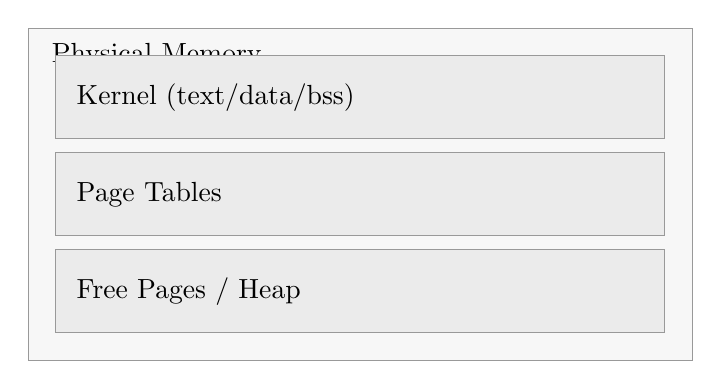
\begin{tikzpicture}[x=1pt,y=1pt]
  \draw[fill=black!3,draw=black!40] (0,0) rectangle (240,120);
  \node[anchor=west] at (5,110) {Physical Memory};
  % Regions
  \draw[fill=black!8,draw=black!40] (10,80) rectangle (230,110);
  \node[anchor=west] at (14,95) {Kernel (text/data/bss)};
  \draw[fill=black!8,draw=black!40] (10,45) rectangle (230,75);
  \node[anchor=west] at (14,60) {Page Tables};
  \draw[fill=black!8,draw=black!40] (10,10) rectangle (230,40);
  \node[anchor=west] at (14,25) {Free Pages / Heap};
\end{tikzpicture}
\end{center}


\end{document}

